\section{\hfil Lab Worksheet VIII \hfil}
\subsection*{Simple regression analysis}
\addcontentsline{toc}{subsection}{Simple regression analysis}

This lab worksheet guides you through the basics of doing simple regression analysis in Stata. The exercise does not really teach you the theory behind regression analysis, instead it focuses on the technical aspect of doing with Stata what you learned in your lectures. If you feel you need a reminder you can look up in the course's materials what regression analysis, regression coefficients, and $R^2$ are. It is also fundamental to know the difference between dependent and independent variables (the latter are also called \textit{predictors} or \textit{regressors}).

The data we are going to use come from the European Social Survey Round 8 (2016) in Great Britain. The dataset is called \textbf{essuk16} and you can find it on LEARN. As we already know, the first step when dealing with new data is to explore them. Use the following commands to find out more about this dataset:

\begin{lstlisting}
	describe
	summarize
	codebook, compact
\end{lstlisting}

These commands are helpful because they tell us things like what the dataset's variable labels mean. Tabulations are useful when exploring data too. Let's see how the data are distributed (remember you can shorten most Stata commands):

\begin{lstlisting}
	tabulate happy
	tabulate trstprt
	tabulate trstplt
	tabulate atchctr
\end{lstlisting}

From the above we want to see things like ``a happiness of 8 out of 10 seems to be the most frequent (about 30 percent)'' or that ``about 60 percent of the British population trust their political parties 4 out of 10 or less.'' We can obtain information from individual variables by using tabulations, but we could also graph the same data:

\begin{lstlisting}
	graph bar (percent), over(trstprt, label(angle(45)))
\end{lstlisting}

The way we explore new datasets partially depends on personal preference, however it ultimately comes down to ``what we need to do'' with the data (perhaps a barplot is more useful if we need to communicate these data to an audience that is not very familiar with tabulations).

Now that you know a bit more about this new dataset, we are going to perform a simple regression analysis. For the sake of this exercise we are going to assume that the following hypothesis is true: \textit{``How happy a person is impacts on their trust in political parties.''} We should also consider a few more things:

\begin{itemize}
	\item If our theory poses that the happier a person is the more trust they will have in political parties, we can expect a positive regression coefficient.
	\item If our theory poses that the happier a person is the less trust they will have in political parties, we can expect a negative regression coefficient.
	\item To verify the points above we need to know how our variables are coded (i.e., ``do they go from least to most?'')
\end{itemize}

We should acknowledge a final note; the two variables we are going to use in our regression analysis are scales, which technically are not continuous but ordered-categorical. Some authors argue that these data can be used in linear regression insofar some assumptions are met. These assumptions are well beyond the scope of this exercise, so we are going to ignore them for simplicity's sake.

To run a simple regression model we type the following in Stata:

\begin{lstlisting}
	regress trstprt happy
\end{lstlisting}

The command \texttt{regress} can be shortened to \texttt{reg}. Remember that you can find out more about any Stata command with the command \texttt{help}. The first variable in our regression command represents our \textit{dependent variable}, whilst the rest of variables (in this case there is only one) are our \textit{independent variables}. In other words, we are assessing the impact of happiness on trust in political parties. Figure 1 below shows the regression output.

\begin{figure}[H]
	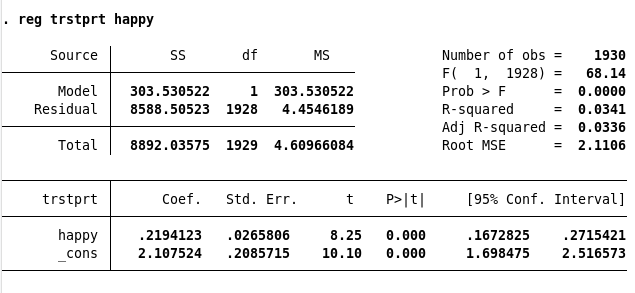
\includegraphics[width=\linewidth]{./img/reg1.png}
	\caption{Simple linear regression with happiness as predictor.}
\end{figure}

We can see that this model was performed on 1,930 respondents (why do you think the model missed 29 people?) The value of $R^2$ is not impressive (a mere 0.034). This figure indicates that 3.4 percent of the variance in our dependent variable (trust in political parties) is explained by the model (which has only one predictor, happiness). The regression coefficient of happiness is statistically significant at the 0.001 level, but the impact seems rather small: for each one-unit increase in happiness we can expect about 0.22 increase in trust. The constant is statistically significant too, and it indicates the value of the dependent variable when all independent variables are zero (in other words, if we were to graph the regression line the constant is the point at which the line would cut the vertical Y-axis). According to this model, our ``starting point'' is of about 2 points of trust.

Perhaps happiness is not the best ``predictor'' of trust in political parties. Let's use this time trust in politicians as a predictor of trust in political parties. We could assume the following (rather redundant) hypothesis: ``people with high levels of trust in politicians will also show high levels of trust in political parties.''

\begin{lstlisting}
	regress trstprt trstplt
\end{lstlisting}

\begin{figure}[H]
	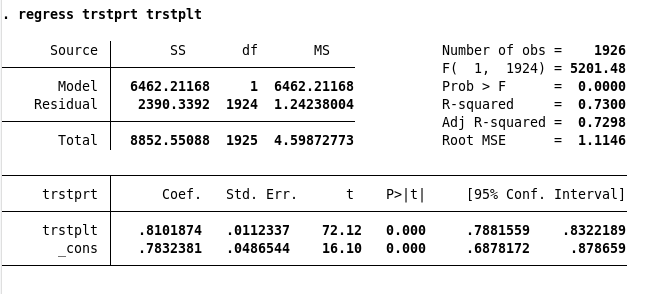
\includegraphics[width=\linewidth]{./img/reg2.png}
	\caption{Simple linear regression with trust in politicians as predictor.}
\end{figure}

We can see several changes. First, the number of observations went down to 1,926. On the other hand, $R^2$ went up drastically to 0.73 (73 percent of the variance in our dependent variable is explained by our model). The value of $R^2$ is very high, and in this case it might be a sign that our variables are really measuring the same thing. The regression coefficient is again statistically significant at the 0.001 level (so we can say with confidence that is different from zero). The coefficient itself predicts an increase of 0.81 in trust in political parties for each unit-increase in trust in politicians, i.e., when trust in politicians increase by 1 we can expect an increase in trust in parties of 0.81. Because both variables are measured using the same scale we can easily see that the change is pretty similar (but not identical).

Let's run one last regression. This time we are going to predict happiness using the age of our respondents. Our research question could well be either ``older people are happier than younger people'' or the opposite.

\begin{lstlisting}
	regress happy agea
\end{lstlisting}

\begin{figure}[H]
	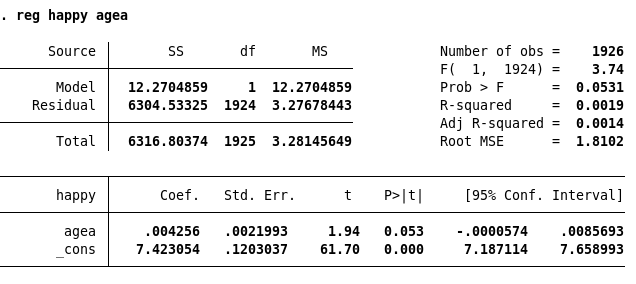
\includegraphics[width=\linewidth]{./img/reg3.png}
	\caption{Simple linear regression with age as a predictor of happiness.}
\end{figure}

Notice the value of $R^2$ (0.0019). According to this model, age accounts for a mere 0.19 percent of the variance (information) in happiness. We can also see that the coefficient is not statistically significant at the 0.05 level (yet just so). The coefficient itself would suggest that a one-unit increase in age results in about 0.0043 increase in happiness. This model is not very useful as it does not explain the variance of our dependent variable very well. Exploring the data before and after performing an analysis is critical to finding issues with the distribution of the data that might account for poor-performing models. For example, we could have plotted the average of happiness for each age to see if there is a pattern:

\begin{lstlisting}
graph bar (mean) happy, over(agea, label(labsize(tiny) angle(45)))
\end{lstlisting}

The resulting graph does not show a clear pattern, and more importantly it does not suggest any linearity at all (remember the ``linear'' in ``linear regression''). Keep in mind that when doing ``real'' linear regression analysis (i.e., not a lab exercise) the technique requires some important assumptions to be true.
